% ======= Welcome to HCoV Skills Workshop 1 =======
%
% You may wish to Share the Overleaf project
% with the others in your group to collaborate.
%
% You should read through this source window to see the
% full instructions for the workshop.
%
% In this workshop we will do some small-scale writing
% exercises and cover some basics of using LaTeX.
%
\documentclass{UoESoMworkshop}
\title{HCoV Skills Workshop 1}

% Replace A, B, C, D below with the names of your group members.
% Then click Recompile (or press Ctrl+S).
\author{A, B, C, D}

\begin{document}
\maketitle

\section{Communication exercises}

Below are two attempts to describe Figure~\ref{fig:completeGraph} in such a way that someone else could reconstruct the figure from just the description.

\begin{figure}[h]
    \centering
    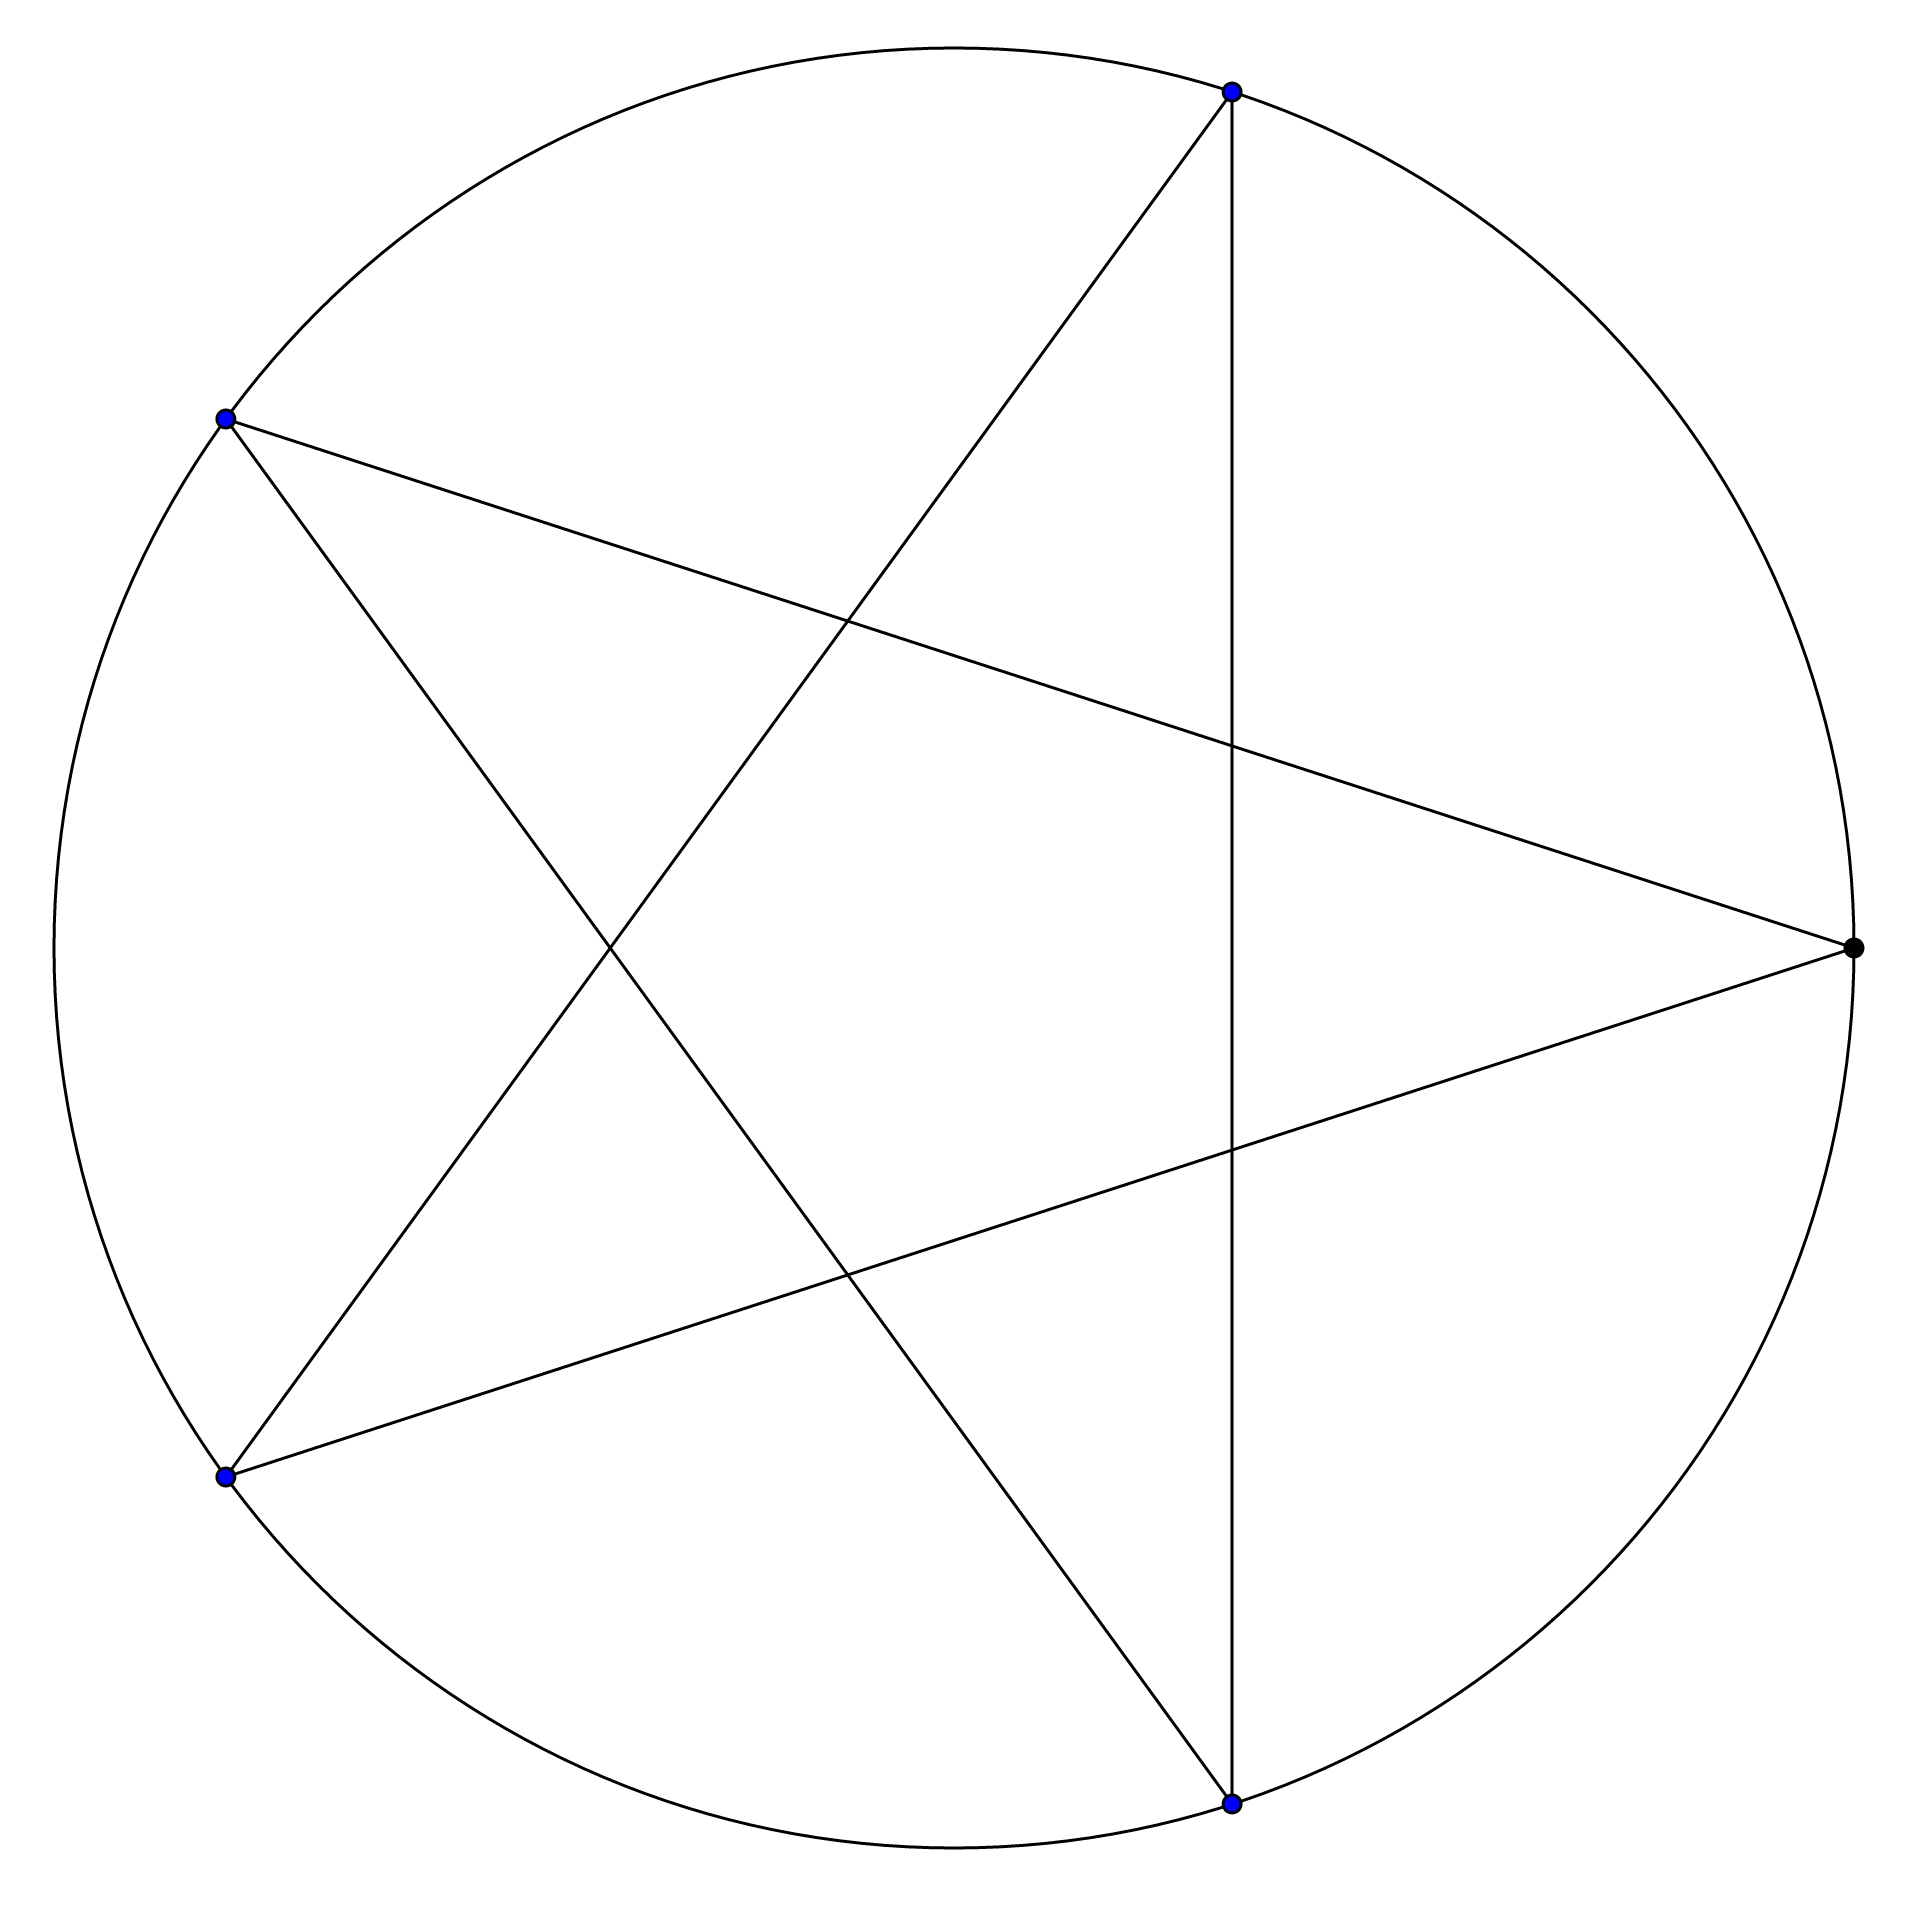
\includegraphics[width=0.35\textwidth]{d9}
    \caption{A complete graph}
    \label{fig:completeGraph}
\end{figure}

\begin{quote}
``The figure consists of a circle on the perimeter of which 
are marked five equally spaced points, one of which is coloured black with the remaining coloured blue. 
Each of these five points is joined to the two points furthest from it by a line segment.''
\end{quote} 

\noindent Or I might try to do it by naming the points: 
\begin{quote}
``The figure consists of a circle on the perimeter of which are marked five equally spaced points $A,B,C,D,E$ in order. 
(The points could be the vertices of a regular pentagon.) Four points are coloured blue and the fifth point is coloured black.
As well as the circle, the diagram contains the line segments $AC$, $BD$, $CE$, $DA$ and $EB$.''
\end{quote} 


\begin{exercise}[10 min]
On your own, take 3 minutes to consider each of the above descriptions. Which do you think is better given that the aim was for someone else to be able to reconstruct the figure from just the description? In what situations might each description be better than the other? Can you improve the descriptions?

Now discuss your views with the rest of your group.
\end{exercise}


\begin{exercise}[15 min]
Work together to write a description of Figure~\ref{fig:d7}. Start with a draft and then agree a final version. 
\end{exercise}

\begin{figure}[h]
    \centering
    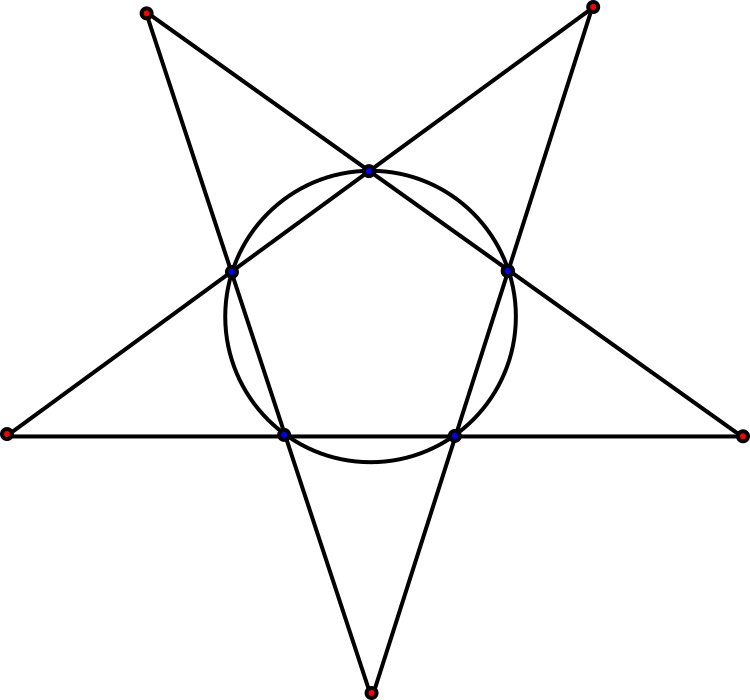
\includegraphics[width=0.6\textwidth]{pent}
    \caption{A figure for you to describe}
    \label{fig:d7}
\end{figure}

% == Type your description in here ===
The figure consists of a pentagon cut from the outside by a circle. The corners of the pentagon are coloured blue. Extend the edges of the pentagon so they intersect at five points, which are coloured red.
% ====================================


\section{Correct the \LaTeX{} code}

\begin{exercise}[15 min]
Correct the LaTeX in this section according to the comments in the source code.

The resources ``Learn LaTeX in 30 minutes'' and ``A quick guide to LaTeX'',
available from the Learn page, may come in handy.
\end{exercise}

\subsection{Using LaTeX}   % This is meant to be a subsection heading

\LaTeX{} is a \emph{logical typesetting language} % LaTeX should be displayed properly (as in the section heading) and the last three words should be emphasised 
so headings such as the one just above should be put in with LaTeX commands. The same applies to lists like the one 
in \ref{math_in_latex}.   % Break the paragraph here
%Also give subsection 2.2 a name using \label and replace the "2.2" by a \ref

The LaTeX referencing system is very powerful and you should use it where possible. It saves a lot of time in the long run. 


\subsection{Mathematics in \LaTeX{}}\label{math_in_latex}  % This is meant to be a subsection heading

% Correct all of the code below so that it appears properly.

Here are three important properties of the complex numbers $\mathbb{C}$.  

(1) If $z$ is a complex number then $|z|=1$ if and only if $z$ lies on the unit circle in the complex plane. 

(2) If $z=x+iy$ and $w=u+iv$ then $$wz= (xu-yv) + i(xv+yu)$$. %that last equation should be displayed on a line of its own

(3) Every polynomial equation with complex coefficients has a solution in the complex numbers.  This is called the ``Fundamental theorem of Algebra''.   % do those inverted commas look right in the output? 

(4) The exponential function can be defined on complex numbers, and
\begin{align*}
    e^{i \theta} = \cos\theta + i \sin\theta
\end{align*}
    So, in particular, 
\begin{align*}
    e^{i\pi}=-1
\end{align*}



\section{Common errors in mathematical writing}

Below are nine examples demonstrating some common errors in 
mathematical writing. What is wrong with each example? How might we improve them? Try to think
of the best way to express the same content rather than just patch up any obvious errors.

\begin{exercise}[20 min]
\begin{enumerate}
\item $a>0$.
\item $2$ is the only even prime.
\item Subtract from both sides of the equation.
\item Multiplication by a negative number on both sides would change the direction of an inequality.
\item An invertible matrics is when the determinant is non-zero. 
\item Plug-in that expression in the other equation.
\item This set of matrixs are all invertible. 
\item It follows $x−1 = y^4$.
\item An important identity is \[ \cos^2x + \sin^2x = 1\]
\end{enumerate}
\end{exercise}


% == Type your improved versions in here ===
\begin{enumerate}
\item The number $a$ is positive.
\item The number $2$ is the only even prime.
\item Subtract from the equation.
\item Multiplication by a negative number would change the direction of an inequality.
\item A matrix is invertible if and only if it has non-zero determinant.
\item Plug that expression in the other equation.
\item This set consists of invertible matrices. 
\item $\implies y^4=x−1$.
\item An important identity is \[ \cos^2x + \sin^2x = 1.\]
\end{enumerate}
% ==========================================



\section{``Microwriting''}
We will practice writing short explanations. We might for instance ask for an 
introductory couple of sentences on complex numbers in no more than 50 words 
and using a minimum number of formulae. A good answer might be as follows. 

\begin{quote}
``A complex number is a new sort of number which takes the form $x+iy$ where $x$ and $y$ are both real numbers. 
The new symbol $i$ is taken to satisfy $i^2=-1$. We add and multiply complex 
numbers just as we would normal algebraic expressions, replacing $i^2$ by $-1$ whenever it occurs.'' 
\end{quote}

\begin{exercise}[20 min]
Summarise in 30 words or fewer the situation concerning how many real solutions a 
real quadratic equation \( ax^2+bx+c=0 \) may have and how this relates to the expression \( b^2-4ac \). 
\end{exercise}

% == Type your summary here ===
The amount of real roots of the real quadratic equation $ax^2+bx+c=0$ depends on $\Delta:=b^2-4ac$. It has two distinct roots iff $\Delta>0$, two identical roots  iff $\Delta=0$, and no root iff $\Delta<0$.


\begin{table}[]
    \centering
    \begin{tabular}{c|c}
    two distinct roots     &  \\
         & 
    \end{tabular}
    \caption{Caption}
    \label{tab:my_label}
\end{table}
% =============================


\begin{exercise}[20 min]
Just as for any other course, 
the University's academic misconduct rules apply in HCoV Skills. See the School guidance at 
\url{https://teaching.maths.ed.ac.uk/main/undergraduate/studies/assessment/academic-misconduct}
and the links from there. 

Write a clear and concise account of what constitutes plagiarism and collusion, and the possible consequences of academic misconduct.
\end{exercise}

% == Type your account here ===


% =============================


\end{document}